\documentclass[fleqn,10pt]{article}

\usepackage[left=2cm,right=2cm,
			top=1.25cm,
			bottom=2.25cm,%
			headheight=11pt,%
			letterpaper]{geometry}
			
\frenchspacing			



\usepackage{multicol}
\usepackage{fancyhdr}
\usepackage{blindtext,graphicx}
\usepackage[absolute]{textpos}
\usepackage[parfill]{parskip}
\usepackage[colorlinks]{hyperref}
\usepackage{hyperref}
\usepackage{gensymb}
\usepackage{csquotes}
\usepackage{amsmath}
\usepackage{fontawesome}
\usepackage{orcidlink}




\usepackage{graphicx}
\graphicspath{ {../media/} }

\usepackage{tcolorbox}
\newtcolorbox{autem}{colback=red!5!white,colframe=red!75!black}
\newtcolorbox{toolchain}{colback=blue!5!white,colframe=blue!40!black!40}
%https://tex.stackexchange.com/questions/66154/how-to-construct-a-coloured-box-with-rounded-corners

%\usepackage[sfdefault,light]{roboto}

\setlength{\TPHorizModule}{1cm}
\setlength{\TPVertModule}{1cm}







\title{On the application of microwave acoustic resonant viral inactivation
\thanks{I would be delighted to include any criticisms or comments anyone may have, both on substance and comprehensibility; preferably leave them on the GitHub issues page, or email therobotist@gmail.com, @0xDBFB7 on Twitter, or irc.0xDBFB7.com:6667 \#covid.}}
\date{May 2020}
\author{Based primarily on exceptional work by }


\begin{document}

\flushbottom 
\maketitle
\thispagestyle{empty}



\begin{textblock}{5}(1,1)
\noindent Please view the latest version at github.com/0xDBFB7/covidinator
\end{textblock}
%\begin{textblock}{5}(1,27)
%\end{textblock}

\null\begin{tabular}[t]{l@{}}
  {Daniel Correia}\ \orcidlink{0000-0002-9353-0216}  \\
  \textit{York University}
\end{tabular}



\begin{abstract}

We extend this landmark work rather trivially by:\\


Aims:

\begin{itemize}
  \item Establishing the time dependence of inactivation
  \item Demonstrating a modulation scheme that decreases the inactivation threshold to below current safety levels in surrogate bacteriophage
  \item Demonstrating a prototype emitter in an "electromagnetic mask" form-factor, costing about \$5 in prototype quantities, which can reasonably be produced in 10 million-of quantities
  \item Testing power thresholds in various conditions; biological fluids of various conductivities and pHs
  \item Using a coarse-grained molecular-dynamics simulation to optimize the impulse
  \item Using a virus-in-the-loop optimization with a centrifugal microfluidic system
  \item Discussing the biological basis for the safety of the device
  \item Showing that the deviation from the expected theshold could be explained by variance in the 
  
\end{itemize}

{Perhaps notable that a completely free and open-source toolchain was used for the entire project, including FDTD microwave antenna optimization. This work can be replicated with \$500 in equipment.}

\end{abstract}


\begin{autem}
	{\large  \it autem} \\
	
	This work was prepared by an undergraduate and has not been peer-reviewed. Additionally, the author has no prior experience with either biology or microwave design. \\

	While our study is very simple, biology is of such complexity that a tremendous amount of care must be taken before any conclusion can be drawn at all. It is not likely that we have taken sufficient care.\\ 

This is especially true with RF biophysics. The literature is littered with otherwise impeccably perormed research which was later demonstrated to be an artifact. \\

	Though the original research used Inf. A, our testing was only performed with a surrogate bacteriophage. All experiments must be repeated with SARS-NCoV-2. \\

	Additionally, other sterilization techniques may produce superior results and should be evaluated in the same context. Data on far UV [Buonanno 2017] indicate safety.\\

It has occurred before that otherwise striking resonances were detected and replication found them to be artifacts of the measurement equipment. [Foster 1987] even offers this disclaimer:

"To detect the DNA resonances with the probe
technique requires correction for system errors that are
potentially much larger than the effect to be studied and
lead to resonance-like artifacts. This is true even with the
more precise instrumentation used in this study. Such data
are easily misinterpreted, and we suggest this might have
happened in the former study."

The direct inactivation plaque and PCR data from [Yang], replicated by [Sun], is a somewhat convincing corroboration that this effect is not an artifact, but hundreds of convincing and  wrong papers exist in the literature. Our data is crude and imprecise, our equipment hastily constructed, and should not be considered validation of this effect even existing. \\


	Please consider all claims with appropriate skepticism.

\end{autem}
	

\begin{multicols}{1}


With typical 2.4 GHz microwave exposure, sterilization occurs by heating of the fluid and tissue.

Of course, the temperature of the atoms of the virus undoubtedly increase; but the 

\begin{toolchain}
	{\it \bf [Yang 2015]'s toolchain}
	\begin{itemize}
	\item Envelope/liposome breaking strength and stiffness from AFM nanoindentation data
	\item Analytical expression assuming homogenous sphere for microwave absorption cross-section
	\item Experimental absorption data from microwave cuvette -> 
	\item COMSOL finite-element for illustration
	\end{itemize}
\end{toolchain}

\end{multicols}






%%%%%%%%%%%%%%%%%%%%%%%%%%%%%%%%%%%%%%%%%%%%%%%%
\clearpage
%%%%%%%%%%%%%%%%%%%%%%%%%%%%%%%%%%%%%%%%%%%%%%%%
\paragraph{\textbf{Time dependence}}\

The chain of literature -> -> 

Both Yang and [] used an apparently arbitrary 15-minute exposure in their tests - a very reasonable decision given the focus of their paper. 

The effectiveness against airborne particles, and to minimize the power required in a dwelling phased-array beam, we must first establish the required duration of exposure.

{\color{red} speculative hypothesizing \{ } 

In contrast to chemical inactivation, where the time dependence appears to be dominated by viscous fluid dynamic effects [Hirose 2017], or UV inactivation, where a certain quantized dose of photons must be absorbed, we expected RF to act instantaneously.

As a damped, driven oscillator, the ring-up time of the virus depends on the Q factor. Yang et al. state the Q of Inf. A as between 2 and 10, so at 8 GHz the steady-state amplitude should be reached in well under 100 nanoseconds.???????????FIXME

[] found a significant mechanical fatigue effect in phage capsids, where a small strain applied repetitively eventually causes a fracture. Such a mechanism could perhaps extend the exposure required to break the capsid or membrane. Other mechanisms could include some sort of lipid denaturation, requiring an absolute amount of energy absorption to break or twist bonds and modify the properties before the envelope fractures.


{\color{red}  \} } 

\footnote{All values have been converted to $W/m^2$ to avoid confusion.}



\clearpage
%%%%%%%%%%%%%%%%%%%%%%%%%%%%%%%%%%%%%%%%%%%%%%%%
\begin{multicols}{1}
{\Large Safety}\\
%%%%%%%%%%%%%%%%%%%%%%%%%%%%%%%%%%%%%%%%%%%%%%%%



Because this is an ostensibly novel and niche mechanism, it may behoove us to breifly review the biological basis for the safety limits set by standards organizations. \footnote{The idea of biological microwave resonances appears to have originated in [Frohlich 1968, 1980].}


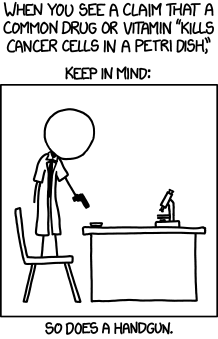
\includegraphics[scale=0.5]{cells.png}


\footnote{Contrary to some [Hardell 2017] reports, we do not find the FCC and ICNIRP to be significantly affected by special interest groups; their rationales appear to be transparent.  [FCC-19-126A1] an FCC memorandum wherein the FCC tells groups to respectfully screw themselves no fewer than three times: ''Similarly, IEEE-ICES urges the Commission to
adopt a higher SAR exposure limit of 2 W/kg averaged over 10 g. [snip] We are not persuaded that the IEC standard should be adopted at this time.", "Medtronic and the AAMI-CRMD recommend a more relaxed threshold of 20 mW. We decline to increase the 1-mW threshold.". Things heating up at the Microwave Safety fandom.}

There are also things.

For instance, it is reasonable to wonder why we might not see such resonances in bodily tissues. Approximately similar nanoscopic structures exist in humans, such as nuclear pores (120 nm) and the famous microtubules (10x50 nm). 

While from which epidemiological data could be derived.\footnote{The cloud service [scite.ai] was irreplaceable during this. It's like a mirror to an alternate universe where literature made sense.}

What we find is a messy affair. Biology is hard.

\rule{\linewidth}{0.2pt}

There are some 20,000 papers on the topic of RF safety, with solid in vitro, in vivo and epidemiological evidence of safety in the 2.4 GHz and 5.8 GHz bands.

However, "There are limited experimental human data upon which to set limits on exposures above 6 GHz" [Chan 2019]. Only 2\% of the above papers are on frequencies $>6$ GHz [Vijayalaxmi 2018]. 

In addition, what data remains in this category is of varying quality. 

As has been starkly demonstrated in the recent hydroxychloroquine contradictions [Gautret 2020] [Geleris 2020], biological research must be essentially perfect to have any meaning at all.


The IEEE standard which the flagship paper [Yang 2015] references [IEEE C95.1-2005] was recently overhauled [IEEE C95.1-2019] with new metrics.


[Vijayalaxmi 2018] is a remarkable meta-analysis of in vitro data. They synthesize a quality score, rating bindedness, sham controls, dosimetry, and sample size. Quality was inversely, monotonically related to the effect size. An example of the subtle effects that can call into question superfically reasonable results are [

They additionally find a publication bias of incredible magnitude in the positive (harm) direction in this field, further degrading the usefulness of statistical analyeses.

An example of a relevant study that they grade as "quality 1" [Karaca 2011]. This study's conclusion is that However, in figure 5, one can see that only 1 out of 11 genes tested had a statistically significant difference in expression. Given the N=6 cultures, 

\rule{\linewidth}{0.2pt}

[Adair 2002] demonstrate theoretically that acoustic resonances are, in general, highly unlikely in biological solvents, primarily focusing on DNA. All resonance modes are strongly overdamped by the surrounding solvent, and no amplitude amplification can take place.

This analysis would seem to disagree with the viral resonance apparently conclusively demonstrated by [Yang 2015] - the PCR result seems especially inarguable. This could be explained by the large charge on the virus compared to the molecules analyzed in Adair. [Yang 2015] find a charge of order $10^7 e$, whereas Adair analyzes a very different regime, "assume coupling to the field through single charges q = e at each end".

[Liu 2009] cite [Edwards, Swicord 1984], saying: "It was proposed that a hydration layer surrounding DNA molecules could lower the viscoelastic transition
frequency, raise the quality factor of confined acoustic vibrations, and result in a microwave resonant absorption". 

But [Adair 2002]'s [Foster 1987] seem to quite conclusively put the kibosh on that idea, demonstrating no resonances in DNA with 20x higher precision than previous work, showing previous results to be an artifact of the measurement equipment.

The supplemental material to [Vijayalaxmi 2018] has a table of studies on this topic. High-quality research in-vitro concurs with.

\paragraph{[Manikowska 1979]} \

9.4 GHz pulsed / in vivo, mouse, $0.1-10 \text{mW}/\text{m}^2$ over the whole body for 2 weeks. N=16.

This is a particularly concerning result, especially given their $p<0.001$. [Servantie 1989] discusses the (admittedly circuituious) route by which birth defects could occur.

Work by [Manikowska 1985] in the 2.4 GHz range has been contradicted [Beechey 1986], but the 9 GHz range does not appear to have been repeated.

\rule{\linewidth}{0.2pt}

More modern research [Juutilainen 2011], [Chemeris], [Vijayalaxmi 2006],  does not tend to agree with these concerns. As cited by [ICNIRP 2020]'s excellent literature review, expose lymphocyte blood cells to 8 ns pulsed 8.2 GHz radiation for 2 hours at an average power of $10 \text{mW/cm}^2$. They find no change in any of the parameters measured, including various chromosomal parameters. They further discuss previous results.

\rule{\linewidth}{0.2pt}

In the frequency range of interest, there seems to be good-quality in-vitro evidence using lymphocytes of lack of harm. We are not aware of any high-quality in vivo or epidemeological data from which useful conclusions can be drawn. 

We must defer to health experts for interpretation of these data.

\rule{\linewidth}{0.2pt}

{\it Please contact the author if you are aware of other salient research, or have a different interpretation.}

\footnote{``{\it{For example, below about 6 GHz, where EMFs penetrate deep into tissue (and thus require depth to be considered), it is useful to describe this in terms of “specific energy absorption rate” (SAR), which is the power absorbed per unit mass $(W/kg)$. Conversely, above 6 GHz, where EMFs are absorbed more superficially (making depth less relevant), it is useful to describe exposure in terms of the density of absorbed power over area $W/m^2$, which we refer to as “absorbed power density”}}'' [ICNIRP 2020 \faExternalLink]}

\end{multicols}















\clearpage
%%%%%%%%%%%%%%%%%%%%%%%%%%%%%%%%%%%%%%%%%%%%%%%%
\begin{multicols}{1}
{\Large Biology}\\
%%%%%%%%%%%%%%%%%%%%%%%%%%%%%%%%%%%%%%%%%%%%%%%%

\paragraph{\textbf{Centrifugal microfluidics}}\

The field of centrifugal microfluidics is accelerating. 

Many CD microfluidics systems use standard CD molding techniques for the channels and machining techniques, using either acrylic or silicone. The turbidity sensor is most sensitive if the plastic is clear. Sterilization does not seem to be discussed. 

Polypropylene is the ideal material, being almost indefinitely autoclavable. It is quite difficult to machine.

\end{multicols}












\clearpage
%%%%%%%%%%%%%%%%%%%%%%%%%%%%%%%%%%%%%%%%%%%%%%%%
\begin{multicols}{1}
{\Large Modes of application}\\
%%%%%%%%%%%%%%%%%%%%%%%%%%%%%%%%%%%%%%%%%%%%%%%%

\paragraph{\textbf{Personal 'electromagnetic mask'}}\

Even with judicious use of phased-arrays, spatial power-combining, etc, each transistor can only reasonably sterilize approx. $ 1 \text{ m}^3 $.

We therefore demonstrate this form factor because, superficially, there are fewer people than there are places. 

On the other hand, a personal device may present issues with participation and production volume. 

\paragraph{\textbf{Direct treatments}}\

[Hand 1982] $E_{mag}=1/e$ (13.5\% power density) skin\footnote{electromagnetic skin, not tissue skin}\footnote{well, both, I suppose.} depth is approximately:

\begin{center}
\begin{tabular}{|l|l|l|}
\hline
F=10 GHz          & Dry tissue & Wet tissue \\ \hline
Penetration depth & 30 mm      & 5 mm \\ \hline
\end{tabular}
\end{center}

SARS is found widely distributed throughout the most favorable organs [Ding 2004], shielded by an average of 4 cm of chest wall [Schroeder 2013]; so safe external treatment of the body is unlikely.

However, destruction of lung tissue appears to be the primary cause of death via SARS [Nicholls 2006]. 

A bronchoscopic technique may therefore be effective, very similarly to that demonstrated by [Yuan 2019]: the bronchi are less than 2 mm thick [Theriault 2018] and the lungs themselves are only on the order of 7 mm thick [Chekan 2016]. 

There is considerable tolerance in the 

Further study is required to validate this method.

\paragraph{\textbf{More fanciful concepts}}\

Many systems operate in these X-band frequency ranges; and precision 

It is relatively easy to produce megawatts of power at these frequency ranges using Klystrons.

Existing marine, weather, and aviation radar systems often use the X-band; depending on the focusing power

\paragraph{}

Finally, there is one concern. Use of this technique will provide a selection bias towards immunity to electromagnetic fields, which could perhaps be effected by preferring extreme-sized mutants (shifting the resonance away from the applied field). We do not have the biological knowledge to know if this is plausible; it is simply worth mentioning.

\end{multicols}







\clearpage
%%%%%%%%%%%%%%%%%%%%%%%%%%%%%%%%%%%%%%%%%%%%%%%%
\begin{multicols}{1}
%%%%%%%%%%%%%%%%%%%%%%%%%%%%%%%%%%%%%%%%%%%%%%%%

\noindent\fbox{\parbox{\linewidth}{
	Toolchain:
	\begin{itemize}
	\item Failed oscillator feedback-loop optimization toolchain: QUCS 0.0.20 + python-qucs + scipy's 'basinhopper'
	\item Successful A slightly modified ngspice + ngspyce + pyEVTK
	\item gprMax for FDTD EM simulation
	\item KiCAD, wcalc, scikit-rf, ngspice
	\end{itemize}
}}
%


The oscillator is a 'wideband double-tuned varactor VCO', based almost verbatim on [Tsuru 2008] and the reference design in Figure 8.36, p378 of [Grebennikov 2007]. 

The rest of the papers in the bibliography were highly enlightening regarding the principles of microwave oscillator design.

This topology of oscillator worked marvellously on essentially the first try. 

The process by which we failed miserably to design our own oscillator topology is detailed in the supplemental.

The following properties: P1dB

For ease of design and simulation, a device with Touchstone S-parameters and SPICE files is greatly preferable.

It is commonly claimed that FR4 is a 'slow' substrate, and that the high loss tangent of ~0.02 makes it unsuitable for microwave systems.

However, with this PCB substrate, the expected loss of only 0.026 dB/mm on signals of minimum 0 dBm is patently acceptable. As viruses do not have a discriminating palate, we are also only minimally concerned with $S_{11}$ reflections, noise, or spurs, so precise impedance control is not required; the wideband VCO sweep accomodates for any variations in resonant frequency due to wide manufacturing tolerances.

As a result of our gross incompetence, the oscillator was designed via an inane, roundabout, and fiendishly tedious manner, and our description of this technique only contributes to the field by being suitable for a dartboard; our analysis can only hold water when combined with paper mache; and a lesser invertebrate in posession of a copy of Microwave Oscillator Design would have accomplished the task faster.

Designing an oscillator of this type in one step with a few kindergarten equations appears to be well within the reach of modern network analytical techniques. Genetic algorithms are quite well matched to this problem, and many commercial software packages are  [computer microwave design book]. 

Initially, 

Not having a good analytical understanding, we resorted to using a purely computational method.

In addition, the design of wideband feedback-loop VCOs is a relatively well-explored field, and many reference designs exist. 

The key sticking point - which we missed - seems to be that at these scales, using microstrip design techniques, the parasitics of any possible filter structure are so large that the small change in impedance that varactors can provide cannot tune the circuit by any meaningful amount.

"Using the lead inductances of the bipolar transistor and varactors provides the required value of the base inductance".

Indeed, [Tsuru 2008]'s "tuned circuit" in Fig 8 is, in fact, just the varactors, plus an almost invisible high-impedance line.





Several analytical filter design methods were 

This is apparently known as a "double-tuned" wideband.

%
\paragraph{\textbf{The feedback loop oscillator}}\

Oscillators must meet the Barkhausen criterion:

\begin{itemize}

\item A 360 degree phase shift around the feedback loop (including the phase shift contribution from the amplifier, which itself varies greatly with frequency)
\item A loop gain $>1.$ 

\end{itemize}\
%
However, a third element is also required:
%
\begin{itemize}
\item A frequency-selective element that restricts oscillation modes and decreases phase noise.
\end{itemize}
%

With large feedback-loop structures, such as long PiN-switched phasing lines, proximity effects from nearby flesh would detune the oscillator significantly.

 design of a triple-tuned oscillator.


\paragraph{}
The buffer amplifiers 

\paragraph{Biasing}\

In our simulations, the varactor-tuned feedback circuit appeared to be particularly sensitive to the introduction of bias-tees. 


The gate must be weakly pulled to ground, otherwise stray charge destroys the oscillation.

\fancyhead[C]{style 1 with thin line}



With 0.79 mm FR4 substrate and 0.2 mm (8 mil) wide traces, the maximum impedance achievable was about 115 ohms, which did not appear to be sufficient as an RF choke. Use of defected grounds can increase inductance, but this was not evaluated.

If suitably high-impedance traces are not available, a common technique is to use a quarter-wavelength line (approximately 6 mm long with the above parameters at 8 GHz) terminated with a stub to produce a virtual short or open circuit [Seo 2007]. 

However, reflections from these structures still appeared to distort the frequency/phase response beyond repair, even with ostensibly wideband stubs [Syrett 1980].

\noindent\fbox{\parbox{\linewidth}{
	Rebuke: despite this blather, many other papers have had success with bias-tees at these frequencies.
}}

Alternate methods evaluated, failures: 


In production, these could be accomodated by graphite-polymer printed resistors. 


Odd-pole varactor-loaded combline filters appeared to have excellent phase and frequency response; however, the geometry necessitates low-inductance via stitching to the ground plane.

%\noindent\fbox{\parbox{\linewidth}{
\begin{autem}
	{\it autem} Others have had great success with varactor-tuned comblines, especially non-grounded lines.
\end{autem}

[Tsuru 2008 fig. 10] is an excellent review of various oscillator designs.

The parasitic inductance of common varactors appears to become problematic at these frequencies (but not for non-wideband use).

\paragraph{\textbf{Spacing}}\

FDTD results still yielded some coupling at 2 mm isolation.

\paragraph{\textbf{Via stitching}}\

Rather than the almost universal technique of via stitching components immediately to the ground plane (a tedious process with our prototyping setup), a large ground pour on the component layer was used wherever ground was needed, as mentioned in [Hunter? combline]. Since we use microstrip rather than coplanar waveguide, 

Since the ground plane does not participate in the DC bias at all, no vias are required in the final device. This means that the drilling, electroless strike and electroplating steps are unnecessary for production.




\clearpage
%%%%%%%%%%%%%%%%%%%%%%%%%%%%%%%%%%%%%%%%%%%%%%%%
{\Large Mass production}
%%%%%%%%%%%%%%%%%%%%%%%%%%%%%%%%%%%%%%%%%%%%%%%%


If this 'electromagnetic mask' form is the ideal (not nearly ), a minimum of 5 GaAs or SiGe:C transistors will be required.

There are, for instance, 1 million hospital beds in the U.S. [AHA 2018]. 

It is difficult to determine the supply capacity for these modern semiconductor processes. A few fermi est

GaAs MMIC market of \$2.2 Bn USD / random sample of MMIC prices = 

3e9 wifi connected devices produced each year.

The largest RFID plants can produce


The techniques and equipment required to produce these are non-trivial. SiGe:C, for instance, requires, 


Figures are not forthcoming, 

Given the supply difficulties of comparatively simple materials such as Tyvek at pandemic scales, it is difficult to imagine that RF semiconductor production can be immediately re-tasked and scaled to this degree. 

\paragraph{\textbf{Vacuum RF triode}}\

One concern is the large filament heater power, which prevents the use of low-cost button cells for power. Use of cold-cathode field-emitter arrays would alleviate this issue, but at the cost of complexity.

Small tungsten incandescent lights are available down to 0.05 watts. With a suitable high-efficiency cathode coating, a pulsed heater power of less than 0.02



\end{multicols}







\clearpage
%%%%%%%%%%%%%%%%%%%%%%%%%%%%%%%%%%%%%%%%%%%%%%%%
\paragraph{Acknowledgements}\
%%%%%%%%%%%%%%%%%%%%%%%%%%%%%%%%%%%%%%%%%%%%%%%%

This paper is not novel enough to deserve this chapter, but those to be acknowledged are.

The authors of the original papers deserve the credit for this entire work;  it is rare that such a monumental finding is served on a silver platter.

Professor Shahramian's excellent video blog {\it The Signal Path} inspired this work. 

Dr. Dainis' videos on microbiological technique were also useful.

Thanks to the professors at York and beyond for returning my emails. 

Thanks to L.H. for wisdom regarding this project.

Thanks to P.B and H.P. for tolerating ramblings and M. for the hug.

Special thanks to all the people - most equally capable of writing this paper if provided the opportunity - who work menial shifts at the component suppliers that remained open that were so critical. Hopfstader be damned; despite the name below the abstract, this paper is of course entirely the result of circumstance and luck. 

Chiefly among the enablers are of course my parents, Doris and Brian, without whom this work would have been done by someone else, and who also supported this work financially. 



One Very Important Thought












\clearpage
%%%%%%%%%%%%%%%%%%%%%%%%%%%%%%%%%%%%%%%%%%%%%%%%
%%%%%%%%%%%%%%%%%%%%%%%%%%%%%%%%%%%%%%%%%%%%%%%%
{\Large Captain's Log, Supplemental}\\
%%%%%%%%%%%%%%%%%%%%%%%%%%%%%%%%%%%%%%%%%%%%%%%%

\paragraph{Molecular dynamics simulation}
\
%\begin{multicols}{1}
%%%%%%%%%%%%%%%%%%%%%%%%%%%%%%%%%%%%%%%%%%%%%%%%

It was originally expected that a large part of this work would be done in-silico, as we did not anticipate having access to suitable RF test equipment. 

Some time was spent attempting to set up a molecular dynamics toolchain capable of simulating an entire virus. 

Having an approximate simulation of the this technique would be useful for a number of reasons: 

We would have a better idea of the transferability to SARS, without wasting the time of experts with BSL-3/4 labs.

The impulse could be subjected to the same optimization as the RF feedback loop. A number of parameters (such as phase, polarization)



Coarse-graining also greatly increases the allowable timestep.


%\end{multicols}




\clearpage
%%%%%%%%%%%%%%%%%%%%%%%%%%%%%%%%%%%%%%%%%%%%%%%%
{\Large Optical centrifuge polarization chirp}\\
\begin{multicols}{1}
%%%%%%%%%%%%%%%%%%%%%%%%%%%%%%%%%%%%%%%%%%%%%%%%







\end{multicols}




\clearpage
\rule{\linewidth}{0.2pt}

There seems to be a discrepancy between [Yang 2015] and our reading of [C95.1-2005].

They use a threshold in open public space of $100(f/3)^{1/5} \text{ W/m}^2$. The 115 W @ 6 GHz they provide correctly corresponds to this equation with a coefficient of 100.

For Table 9, general public, the equation is $18.56 (f)^{0.699} \text{ W/m}^2$, or $64.93 \text{ W}/\text{m}^2$ @ 6 GHz. 

Different versions of the IEEE standard have used equations of equivalent form but with different coefficients [Wu 2015]; it is very possible that we have retrieved the wrong standard.

\rule{\linewidth}{0.2pt}

CEL did not supply a SPICE model for the GaAs FET device used in early prototypes. A FET was originally because a gate is ostensibly easier to bias than a base; but this turned out to be unfounded.

[Steenput 1999] has an interesting analytic method to synthesize a SPICE model suitable for a transient simulations from S-parameter measurements using negative resistances. However, this neglects the I/V characteristic. 

[Polyfet 1998] describes a simple optimization method to synthesize a SPICE model for an active device, and CEL appnote provides some details for GaAs devices.



\rule{\linewidth}{0.2pt}

OpenEMS is excellent, with Python bindings, some lumped components, and mesh refinement. However, embarassingly, we were not able to resolve all the dependency issues in order to install it.

\rule{\linewidth}{0.2pt}

The oscillator design is a testament  This highlights that a computation is not a substitute for understanding.


We began experimentally by building a scaled version of [Mueller 2008]'s active antenna crudely with copper tape, using a CEL [] FET.



We then manually tried a number of filter designs, using the manufacturer's S-parameters and QUCS' microstrip approximations. This intially appeared to yield good agreement with experiment. Peaks in the feedback voltage simulation corresponded approximately with peaks in the observed spectrum. [figures from LO prototype N]. 

A crude, inane, and extremely disorganized trial-and-error procedure was performed for many weeks. A wide variety of analytical methods for filter design were attempted, but simultaneously obtaining the correct phase shift and frequency response was somewhat difficult. The parasitic inductance of the varactors always seemed to destroy our most perfect creations.

An SIR filter has the added advantage of confusing epidemiologists greatly.

Eventually, QUCS, zonca/python-qucs, and scipy's basinhopper was used with the cost function somewhat similar to that described in [Kaplevich]:

\begin{verbatim}
    freq_coeff = 1
    phase_coeff = 1.5
    ratio_coeff = 0.5
    insertion_loss_coeff = 0.2
 
    frequency_cost = freq_coeff * (abs(desired_center_frequency-fb_peak_frequencies[0])/1e9)
    phase_cost = phase_coeff * abs(1.0 - phase_at_peak)
    ratio_cost = ratio_coeff * fb_peak_ratio
    insertion_loss_cost = insertion_loss_coeff*(1.0 - fb_peak_values[0])
    cost = frequency_cost + phase_cost + fb_peak_ratio + insertion_loss_cost
\end{verbatim}

Optimizing first for the high frequency, fixing the inductor and microstrip values, and then optimizing for the varactor values at the low frequency.

This produced a seemingly acceptable feedback loop:

\includegraphics[scale=1]{LO_2_pole_test.png}

However, when this was built, varactor tuning performance was abysmal, with hops and peaks; and the tuning range was far smaller than expected.

It was thought that a transient simulation - to determine how the spectrum actually evolved - would improve the situation. 

As of 0.0.20, QUCS' microstrip models are not yet compatible with transient simulations; and some improved filter designs required simulating coupling between more than two microstrips, which QUCS did not yet support natively.

\includegraphics[scale=0.5]{3d_spectrum_2.png}

The complete transient simulation matched reality very closely. 




Because we lacked a spectrum analyzer that could monitor the higher poles of the filter until the bootstrap LO was designed, we had to rely on in-silico analyeses.


Transient simulations with ngspice matched experiment far more closely.

\rule{\linewidth}{0.2pt}

Again, inductive choke biasing in the feedback loop was practically impossible. Biasing PiN diodes with a 10kohm resistor, (with 330 ohm safety resistor) one to 48V bias and another through an 2N7002P N-channel mosfet worked fine. 

The oscillator ran fine with a PiN bias of 2.34 mA. [LO prototype N]. A high bias voltage of 48V was required to get sufficient current through the two 10K resistors and the PiN diode to obtain a low impedance while remaining delicate with the vfb.

The PiN diode used has a resting resistance of 500 ohms, 5 ohms at 2 mA and 2 ohms at ??. 

48V is a little tight on the 50V rated voltage of our DC blocking capacitors.

Each activated PiN diode should be biased separately, since putting 2x 2 mA through 20K would take an impractical 80V.

\rule{\linewidth}{0.2pt}

Conductors are represented by zeroing all components of the electric field in those regions. 

There are many different possible source geometries, each introducing their own distortions.

There are many ways of linking SPICE and FDTD. 

\rule{\linewidth}{0.2pt}

Bandpass filters can be designed by first designing a low-pass filter prototype (usually Chebychev) (or, in our case, using reference filter component tables), and then transforming this low-pass into a band-pass. [Hunter 2001] is an excellent overview of this process, with many design examples for different filter topologies. 

The coupling coefficient between two low-pass filters determines the band-pass bandwidth.[Hui 2012]

[Hunter 2001] also describes an analytical method to create a filter with the precise group delay - phase shift versus frequency - required for stable oscillation. However, simultaneously compensating for the group delay introduced by the amplifier itself (nearly 180 degrees over the frequency range for the CEL part) seemed complex.

Phase shift can be introduced either via a length of microstrip, or a high-pass/low-pass filter [Microwave101]. Adding a fixed microstrip line restricts the tuning range, however, and the filter inevitably affects the frequency response.  

\rule{\linewidth}{0.2pt}

NGSPICE's KSPICE coupled transmission lines require the capacitance and inductance per unit length in Maxwell matrix form, rather than the physical $C_{even}$/$L_{even}$ (each line's capacitance and inductance to ground) and $_{odd}$ (between elements) form provided by tools like wcalc. "matrix not positive definite". [Schutt-Aine] discusses this; we reproduce here for convienience.

\[ L_{11} = L_{22} = L_{even}  \]
\[ L_{12} = L_{21} = L_{odd}  \]
\[ C_{11} = C_{22} = C_{even}+C_{odd}  \]
\[ C_{12} = C_{21} {\it{(unused)}} = -C_{odd}  \]

\rule{\linewidth}{0.2pt}

In practice, the timestep required to obtain convergence in particularly tight corners of the SPICE simulation can drop to 1e-20, which is far below the Courant limit of the FDTD simulation. To eek out a bit more performance, a simple adaptive-timestep technique from [ a ] is used; we simply set the timestep so that the maximum change in voltage per timestep from the non-FDTD portion is less than some threshold.


\rule{\linewidth}{0.2pt}

Originally tried 

The impedance of an antenna over frequency can be determined by:

\begin{itemize}
  \item Applying a gaussian pulse to a voltage source - in our case, applied to a via connecting the path (or probe)
  \item Running the simulation until the transients have all died out below some threshold, while logging the source voltage and current at each timestep
  \item Taking the fourier transform of the (real) excitation voltage and current (producing a complex result, mind you)
  \item Taking the ratio of the two complex spectra.
\end{itemize}

This is the computational equivalent of dropping a piano off a balcony to see which key is stuck.

See [Penney 1994], [Luebbers 1992], [Luebbers 1991], [Luk 1997]. 

Our implementation is in electronics/simple\_fdtd/runs/U.py.

A similar mismatch to the SPICE exists for fourier methods - but in the other direction.  The courant limit often demands fine timesteps, but since each FFT bin is $ f_{bin} = n_{bin} / (N_{simulation} \ dt) $ , the majority of the FFT bins exist into the hundreds or thousands of GHz, leaving no resolution in the low-frequency domain of interest unless $N_{simulation}$ is extremely large - even if all the transients in the simulation have died down, you still have to keep the sim running to make the FFT happy! 

There's more than enough 'information entropy' in 2000 FDTD points for most antennas. But you need some 30,000 points to get 10 bins below 20 GHz!

There are a few methods of changing the FFT bin size artificially, which [Bi 1992] reviews. You can "use a manual fourier integration over the frequency region of interest".

But, in a staggering turn of events which will presumably be familiar to statisticans and preposterous to everyone else, a far simpler method is to {\it discard} 95\% of the data, by down-sampling to 1/10th or so.

An equally simple method that seemed to produce better results in our case is to pad the voltage and current samples to the correct length. The jump discontinuity introduced by padding with zeros has a negligible effect.

It's so thumpingly unintuitive to me that adding 50,000 zeros to a 5000 value dataset can improve the resolution of a measurement by 300-fold.

It is important to remember to normalize the gaussian pulse, or else numerical noise will be introduced. The magnitude is not important - [Luebbers 1992] use 100v, others use 1v, etc.

Though uneven dt FFTs exist, the time step can be constant at the courant limit for this simulation.

A step impulse (1 first timestep, 0 otherwise) has been used in some works, though in our case performance was quite horrid.

A correction factor due to the staggered magnetic field of the Yee lattice must be introduced; [Fang 1994]. Their $Z_2$ equation (correcting for spatial inaccuracies, but not temporal) was sufficient.

A method of moments solver like NEC-2 may have provided faster results; but handling of multiple dielectrics does not seem to be simple.

This technique is equivalent to that used in electrochemistry, known as fourier impedance spectroscopy - except they seem to usually use a known impedance source rather than a hard source, presumably because ideal hard sources don't exist in reality.

Allowing the simulation to run for long enough that all transients dissipate is important for accuracy - deceptive dips in the current can cause early termination. A surprising amount of detail is contributed by even the smallest current levels. Our threshold is 1e-7 amps for 700 iterations.

[Samaras 2004] has a very useful set of experimental and FDTD data for calibration and comparison. Comparing a probe via source in the different positions, we obtained agreement of $\sim 7\%$ in impedance and $\sim 5\%$ in frequency.

The use of a hard source feed-port affects the number of timesteps required by introducing unphysical transients. Using a port with a virtual 50-ohm resistance reduces the computational requirements by a large factor; see [Luebbers 1996].

Simply monitoring the source current during the simulation is somewhat deceptive. Periodically monitoring the change in the fourier transform seems to be a better convergence metric.



\rule{\linewidth}{0.2pt}

Many equations in papers on the FDTD method are supplied without explicit scaling factors. For instance, for use with flaport/fdtd the H-field to current line integral in [] requires scaling by $\mu_0  (dx/dt)$, where $\mu_0$ is the vacuum magnetic permittivity, dx the cell size, and dt the timestep - despite the equation already possessing a deceptive set of $dx$-es.

Naturally, if one is competent, this discrepancy will be immediately obvious. Those not dimensionally-intuitive, such as myself, find it useful to run a test using a unit-aware calculator such as {\it sharkdp/insect}.

\rule{\linewidth}{0.2pt}

The impedance of a microstrip antenna varies with position on its plane. Probe feeds that couple a microstrip to a specific point are often used.

\rule{\linewidth}{0.2pt}


\label{para}
\ref{para}

\paragraph{Timeline}

\paragraph{Comments by others}

\paragraph{Lessons Learned} \


\rule{\linewidth}{0.2pt}

It may be helpful to think of simulations very similarly to IRL experiments. 

A simulation is just a universe in a bottle that you can examine more closely; as with real-world, you can learn much from observation, but 

But this need for documentation conflicts with the rapid, iterative cycle necessary for productivity.

This is obvious to all compentent, but when rapidly iteratively testing with simulations, it may be helpful to automatically save a package with images of all the components (schematics, graphs, input files) of each distinct test. 

For comparison to experiment, having a webcam take an image of the assembled board is also helpful. 

Version control alone isn't quite enough. Just having a simulation setup file somewhere in the commit history isn't "discoverable" - that is, you must be able to see what the input and output was without re-running the simulation. 

Manually taking notes tended to disrupt the flow of testing; and in any case, just noting "SIR filter has appropriate phase response" is almost useless. What {\it was} the phase response? Plot it!

Software such as Sumatra, Sacred, recipy, and others. In our case, we used eLabFTW's elabapy bindings.

\rule{\linewidth}{0.2pt}

It is far easier to use existing, well-characterized reference designs verbatim than to modify 

\rule{\linewidth}{0.2pt}

When rapidly testing data analyses which aren't really conducive to unit testing, I previously used to run the whole simulation, look at the analysis, re-run the sim, etc.

This is slow. I often don't change the input parameters for the sim, but just the analysis. However, there's often a large amount of state to persist to disk.

Saving the entire session with 'dill' is very helpful.

\rule{\linewidth}{0.2pt}

Software opacity is evil.

\rule{\linewidth}{0.2pt}

A great deal of time was spent trying to resolve version conflicts and dependency hells with the numerous libraries used by all the simulation programs. Over a week was spent trying to recursively track down all the This also wastes developer time - some fraction of issues raised are due to library version conflicts. 

Packaged binaries help this slightly, but of course don't help if modifications are required, and managing shared libraries is still a tricky matter.

Good solutions include OpenFOAM's Docker installation. In some cases, using chroot with the original developer's Linux distribution is also of some utility.

But this all seems like quite a lot of overhead and opacity for what ultimately doesn't seem a super-complex problem: deterministically obtain a known-good version of a library, build locally, and set paths appropriately.

A good example might be gTest's cmake integration.

In the extreme, systems exist to extract every 

In some situations (especially where the library has a permissive licence) perhaps it could be useful to consider packaging a complete, batteries-included 'known good' repository, either with the source of all the correct library versions included, or with a script to clone and compile the specific version used, integrating all the libraries with the build system. 

For instance, this was done with the PDB reader in the OpenMM wrapper and JAMES.

\rule{\linewidth}{0.2pt}

There's also a very neat thing that seems to be common in computational biology, but which doesn't seem popular in other fields. After an algorithm or software tool is written (and the source published seperately), a simple CGI frontend is written around it and hosted on the university's servers. eLNemo and the CHARMMing web interface are advanced examples of this. This way, anyone with an input file can get results without futzing around with installation. 

The computational biologists have beat us at our own game.

\rule{\linewidth}{0.2pt}


Write a paper to be understood; to be as clear and helpful as possible to the reader.

\rule{\linewidth}{0.2pt}

We have always encountered wasting extreme amounts of time on subtle assembly mistakes in hardware prototypes. 

In one example in this project, many hours were wasted because the enamel insulation on a bodge wire had not burned off completely in the solder joint, leading to a high-impedance connection.

The same has occurred in previous projects; in one example, many days were spent debugging software to fix an apparently slow hardware interrupt, which ended up being the result of a poor solder paste stencil leading to a hidden high-impedance connection to a leadless package.

Many failures are perhaps the result of carelessness in modification and a lack of inspection; but others would only have been found by a 100\% electrical test.

If flying-probe or bed-of-nails tests can be made sufficiently rapid and closely coupled with the existing toolchain, 

In {\it 2001: A space odyssey}, an automated system is shown guiding the troubleshooting of an assembly, apparently generating a fault tree of all the 

Boundary-scan features might really help 

\rule{\linewidth}{0.2pt}

The ability to almost immediately compare simulation to experiment was quite important.

\rule{\linewidth}{0.2pt}


\paragraph{Hall of Hubris} \

Lest our hats stop fitting

\rule{\linewidth}{0.2pt}

An inane remark:

\begin{displayquote}
We believe once we have the P. Syringae host, we from environmental samples
\end{displayquote}

Truly the depths of Dunning-Kruger.

\rule{\linewidth}{0.2pt}

An expert and distinguished gentleman that we contacted regarding assistance resolving transients in our microstrip VCO stated the following:



This was a perfectly sensible remark; it is almost always the case that (at X-band, no less!) a custom IC would have been needed to build a VCO.

Also, if taken in the context of a tired, overworked PI getting an unsolicited email from an excessively verbose undergraduate at a different university, I hardly think I would have replied differently.

However, I think this person may have missed out. Learning 

So perhaps it is wise to ponder the ideas of fools for skeet; one always learns target practice, if only an example what not to do, and occasionally one learns positively. I have often found that I learn greatly from working on the projects of others.

We present this only as a cautionary tale in the hopes that someday I will listen.

\rule{\linewidth}{0.2pt}

%\end{multicols}

\Acrobatmenu{GoBack}{Back}
\end{document}
